\documentclass{beamer}
\usepackage[utf8]{inputenc}
\usepackage[OT1]{fontenc}
\usepackage[ngerman]{babel}
\usepackage{lastpage}
\usepackage{tikz}
\usepackage{lmodern}
%\usepackage{libertine}
\usepackage{tabularx}
\usepackage{hyperref}
\usepackage{xifthen}
\usepackage{multicol}
\usepackage{tikz}
\usetikzlibrary{positioning}
\usetikzlibrary{arrows}

\newcommand{\n}{\hfill\\\vspace{0.25cm}}

\renewcommand\footnoterule
{
	% Original implementation just with gray color
	\color{gray}
	\kern-3pt 
	\hrule width 2in 
	\kern 2.6pt
}
\renewcommand\thefootnote{\tiny\textcolor{gray}{\arabic{footnote}}}
\let\oldfootnote\footnote
\renewcommand{\footnote}[1]
{%
	\oldfootnote
	{
		\tiny
		\textcolor{gray}{#1}
	}%
}
\newcommand{\citewiki}[2][]
{%
	\footnote
	{
		\ifthenelse{\isempty{#1}}
		{
			Quelle: \href{https://de.wikipedia.org/wiki/#2}{Wikipedia:#2}
		}
		{
			Quelle: \href{https://de.wikipedia.org/wiki/#2}{Wikipedia:#1}
		}
	}
}
\newcommand{\citeurl}[2]
{%
	\footnote{\ Quelle: \href{#1}{#2}}
}
\newcommand{\money}[1]{
	\node
	[
		fill=green!45!gray,
		minimum height=0.4cm,
		minimum width=0.9cm,
		inner sep=0pt,
		rounded corners=0.1cm,
		draw=green!50!black,
		thick
	] at #1 {\scriptsize\color{white}€};
}
\newcommand{\smallmoney}[1]{
	\node
	[
		fill=green!45!gray,
		minimum height=0.3cm,
		minimum width=0.675cm,
		inner sep=0pt,
		rounded corners=0.075cm,
		draw=green!50!black,
		semithick
	] at #1 {\tiny\color{white}€};
}

\input{../flat-blue-theme.inc}

\setbeamercovered{invisible}
\beamertemplatenavigationsymbolsempty

\author[Hauke Stieler]{Hauke Stieler\\\href{mailto:4stieler@informatik.uni-hamburg.de}{4stieler@inf}}
\title{Steuern}
\date{\today}

\begin{document}
	{
		\setbeamertemplate{footline}{}
		\begin{frame}
			
\includegraphics[width=\paperwidth,trim=2cm 2cm -1.9cm 3.35cm]{images/tax-government}
		\end{frame}
		\addtocounter{page}{-1}
	}

	{
		\setbeamertemplate{footline}{}
		\setbeamertemplate{headline}{}
%		\setbeamertemplate{background}{
\includegraphics[width=\paperwidth,trim=0 0 0 3.5cm]{images/tax-government}}
		\maketitle
		\addtocounter{page}{-1}
	}
	
	\begin{frame}{Disclaimer}
		\begin{center}
			Diese Präsentation inklusive Vortrag ist keine Rechts-, Steuer- oder Finanzberatung!\n
			Es besteht keinerlei Garantie für die Richtigkeit der Informationen in dieser Präsentation, alle Angaben ohne Gewähr!\n
		\end{center}
	\end{frame}

	\begin{frame}
		\begin{center}
			Was für Vorwissen hast du?
			% TODO was hier machen? Umfrage? Welche Fragen?
		\end{center}
	\end{frame}

	\begin{frame}
		\tableofcontents[hidesubsections]
	\end{frame}
	
	\section{Basics}
	
		\begin{frame}
			\tableofcontents[currentsection,hideallsubsections]
		\end{frame}
	
		\subsection{Wieso? Weshalb? Warum?}
	
			\begin{frame}{Was sind Steuern?}
				\begin{itemize}
					\item Zahlungen an Staat/Land/Gemeinde
					\item Kein Anspruch auf Gegenleistung
					\begin{itemize}
						\item Anders als bei Abgaben, Gebühren, Maut, etc.
						\item Beispiel: Fahrräder dürfen auf Straßen fahren, obwohl es keine Fahrradsteuer gibt (sondern nur eine Kfz-Steuer)
					\end{itemize}
				\end{itemize}
			\end{frame}
		
			\begin{frame}{Warum eigentlich Steuern?}
				\textbf{Staatshaushalt} decken.
				\begin{itemize}
					\item \href{https://www.bundeshaushalt.de/DE/Bundeshaushalt-digital/bundeshaushalt-digital.html}{bundeshaushalt.de}
					\item Straßen, Eisenbahn, ÖPNV, Zuschüsse zur Rente, Bildung, BAföG, Wettervorhersage, sämtliche Ämter/Verwaltungen
				\end{itemize}
			
				\textbf{Lenkung} von Verhalten (z.B. Tabacksteuer \textrightarrow\ Leute sollen weniger rauchen)
				
				\textbf{Umverteilung} von reich zu arm
			\end{frame}
		
			\begin{frame}{Von wem an wen werden Steuern gezahlt?}
				Steuerzahler zahlt Steuern an Bund/Land/Gemeinde:\n
				
				\begin{description}
					\item[An Bund] Einkommenssteuer, Lohnsteuer, Umsatzsteuer
					\item[An Land] Erbschaftssteuer, Lotteriesteuer, Biersteuer
					\item[An Gemeinde] Grundsteuer, Hundesteuer
				\end{description}
			\end{frame}
		
		\subsection{Grundsätze}
	
			\begin{frame}{Maxime im Aufbau von Steuern}
				\begin{description}[labelwidth=0cm]
					\item[Gerechtigkeit] Nur wirtschaftliche Faktoren wichtig (nicht z.B. Hautfarbe)
					\item[Gleichmäßigkeit] Kein Spielraum/Willkür
					\item[Rückwirkungsverbot] Steuergesetze dürfen nicht rückwirkend in Kraft treten
					\item[Ergiebigkeit] Steuern sollten Staatshaushalt decken + keinen zu hohen Verwaltungsaufwand erzeugen
					\item[Unmerklichkeit] Steuererhebung und -belastung sollte man nicht merken
					\item[Praktikabilität] Steuergesetze sollen transparent, bestimmt und einfach sein
				\end{description}
			\end{frame}
	
	\subsection{Steuersatz}
	
		\begin{frame}
			Der Steuersatz (prozentualer Wert) kann sich wie folgt entwickeln:\n
			\begin{description}
				\item[Proportional] Immer gleicher Prozentwert (z.B. 19\% Umsatzsteuer)
				\item[Progressiv] Prozentwert steigt mit Bemessungsgrundlage (z.B. Lohnsteuer)
				\item[Regressiv] Prozentwert sinkt mit Bemessungsgrundlage \vspace{0.1cm}\newline
				{\tiny Existiert in Deutschland nicht; In USA/UK sind Sozialabgaben regressiv\\}
				\item[Stufen] Prozentwert verändert sich Stufenweise
			\end{description}
		\end{frame}
	
	\section{Glossar}
	
		\begin{frame}
			\tableofcontents[currentsection,hideallsubsections]
		\end{frame}
		
		\subsection{Glossar}
		
			\begin{frame}
				\begin{description}[labelwidth=0cm]
					\item[Steuerschuldner] Gesetzlich Verpflichtet Steuern zu zahlen
					\item[Steuerträger] Wirtschaftlich belastet\citewiki{Direkte\_und\_indirekte\_Steuer}
					\item[Steuerzahler] Person, die tatsächlich das Geld überweist\citewiki{Steuerzahler}
					\item[Veranlagung] Ermittlungsverfahren + Festsetzungsverfahren\citewiki{Veranlagung\_(Steuerrecht)}
					\item[Steuerfestsetzung] Verwaltung stellt Steuerbescheid aus\citewiki{Steuerfestsetzung}
					\item[Steuerbescheid] Zettel auf dem steht welche Steuern anfallen\citewiki{Steuerbescheid}
					\item[Bemessungsgrundlage] Wert auf dem Steuer basiert (z.B. zu versteuerndes Einkommen)\citewiki{Bemessungsgrundlage\_(Steuerrecht)}
				\end{description}
			\end{frame}
	
	\section{Steuerarten}
	
		\begin{frame}
			\tableofcontents[currentsection,hideothersubsections]
		\end{frame}
	
		\subsection{Direkte / indirekte Steuern}
		
			\begin{frame}
				\begin{tabularx}{\linewidth}{X|X}
					\multicolumn{1}{c|}{\textbf{Direkt}} &
					\multicolumn{1}{c}{\textbf{Indirekt}} \\[0.25cm]
					Schuldner = Träger & Schuldner $\neq$ Träger \\
					\vspace{0.25cm}Beispiel Lohnsteuer: \newline
						Ich (Schuldner) muss von meinem Lohn Steuer \textbf{direkt} ans Finanzamt zahlen. Meist vom Arbeitgeber übernommen, es ist aber \textbf{mein Geld}, das überwiesen wird, ich (Träger) trage die Steuerlast selbst. & 
					\vspace{0.25cm}Beispiel Mehrwertsteuer: \newline
						Kunden (Schuldner) zahlen Steuern \textbf{indirekt}, da Verkäufer (Träger) diese auf \textbf{seine Einnahmen} zahlen muss \textrightarrow\ Steuer ist daher im Preis mit enthalten = Kunde \textbf{trägt} die Steuerlast.
				\end{tabularx}\\
				\citewiki{Direkte\_und\_indirekte\_Steuer}
			\end{frame}
		
		\subsection{Personen- / Realsteuer}
		
			\begin{frame}
				\begin{tabularx}{\linewidth}{X|X}
					\multicolumn{1}{c|}{\textbf{Personensteuer}\citewiki{Personensteuer}} &
					\multicolumn{1}{c}{\textbf{Realsteuer}\citewiki{Realsteuer}} \\[0.25cm]
					Steuer \textbf{abhängig} von persönlichen Umständen (Alter, Familie, etc.). & Steuer \textbf{unabhängig} von Personen. \\
					\vspace{0.25cm} Beispiel: Lohnsteuer &
					\vspace{0.25cm} Beispiel: Grundsteuer
				\end{tabularx}
			\end{frame}
		
		\subsection{Quellen- / Veranlagungssteuer}
		
			\begin{frame}
				\begin{tabularx}{\linewidth}{X|X}
					\multicolumn{1}{c|}{\textbf{Quellensteuer}\citewiki{Quellensteuer}} &
					\multicolumn{1}{c}{\textbf{Veranlagungssteuer}\citeurl{https://www.steuererklaerung-verstehen.de/lexikon/veranlagungssteuer}{steuererklaerung-verstehen.de}} \\[0.25cm]
					Steuer wird sofort direkt an Quelle erhoben. & Steuer wird zu anderem Zeitpunkt (z.B. Steuererklärung im Folgejahr) erhoben.\\
					\vspace{0.25cm} Beispiel Lohnsteuer:\newline
						Arbeitgeber (Quelle) überweist mir meinen Lohn und meine Lohnsteuer ans Finanzamt. &
					\vspace{0.25cm} Beispiel Umsatzsteuer:\newline
						Umsatzsteuer wird im Voraus entrichtet, nicht erst, wenn Einnahmen entstehen. Daher ist nach Jahresende eine Steuererklärung Pflicht.
				\end{tabularx}
			\end{frame}
		
		\subsection{Pauschal- / Individualsteuer}
		
			\begin{frame}
				\begin{tabularx}{\linewidth}{X|X}
					\multicolumn{1}{c|}{\textbf{Pauschalsteuer}} &
					\multicolumn{1}{c}{\textbf{Individualsteuer}} \\[0.25cm]
					Steuersatz (Prozent-Zahl) immer gleich. & Steuersatz individuell von persönlichen Verhältnissen.\\
					\vspace{0.25cm} Beispiel Umsatzsteuer:\newline
						Immer 7\% bzw. 19\%. &
					\vspace{0.25cm} Beispiel Lohnsteuer:\newline
						Steuersatz abhängig von Gehalt.
				\end{tabularx}
			\end{frame}
	
	\section{Einkommen und Steuern}
	
		\begin{frame}
			\tableofcontents[currentsection,hideallsubsections]
		\end{frame}
	
		\subsection{Muss ich Steuern zahlen?}
		
			\begin{frame}{Arbeit und Steuer}
				\begin{itemize}
					\item Steuer-Identifikationsnummer (bleibt ein Leben lang gleich)
					\item Arbeit: Selbstständig oder nichtselbständig?
					\begin{itemize}
						\item Selbstständige Arbeit: Selbstständige (Freelancer/Freiberufler, Unternehmer)
						\item Nichtselbständige Arbeit: Angestellte (Werkstudent, "`normale"' Festanstellung)
					\end{itemize}
				\end{itemize}
			\end{frame}
		
			\begin{frame}{Arbeit und Steuer}
				\begin{tabularx}{\linewidth}{X|X}
					\multicolumn{1}{c|}{\textbf{Selbständig}} &
					\multicolumn{1}{c}{\textbf{Angestellt}} \\[0.25cm]
					\begin{itemize}
						\item Schreibt Rechnungen
						\item Umsatzsteuer
						\item Steuererklärung \textbf{Pflicht}
					\end{itemize} &
					\begin{itemize}
						\item Festes Gehalt
						\item Einkommenssteuer
						\item Steuererklärung \textbf{Optional}
					\end{itemize}
				\end{tabularx}
			\end{frame}
		
		\subsection{Wie viel Steuern muss ich zahlen?}
		
			\begin{frame}
				\begin{center}
					
\includegraphics[width=0.75\linewidth]{images/tarifzonen}
				\end{center}
			\end{frame}
			
			\begin{frame}{Steuersätze}
				\begin{itemize}
					\item Einnahmen $\neq$ Einkünfte $\neq$ Einkommen $\neq$ zu versteuerndes Einkommen {\tiny (Trivial!)}
					\item Wie viel Steuern muss ich jetzt zahlen? ... well
					\begin{itemize}
						\item Steuersatz nach Zonen (je nach Einkommen)
						\item Grenzsteuersatz: Steuersatz auf den \textit{nächsten} Euro
						\item Durchschnitssteuersatz: Steuersatz bezogen auf den gesamten Betrag
					\end{itemize}
				\end{itemize}
				Ja aber wie viel ist das jetzt? Hä, na so viel\citewiki[Einkommenssteuer]{Einkommensteuer_(Deutschland)\#Tarif_2020}:
				\begin{center}
					\only<1>{
						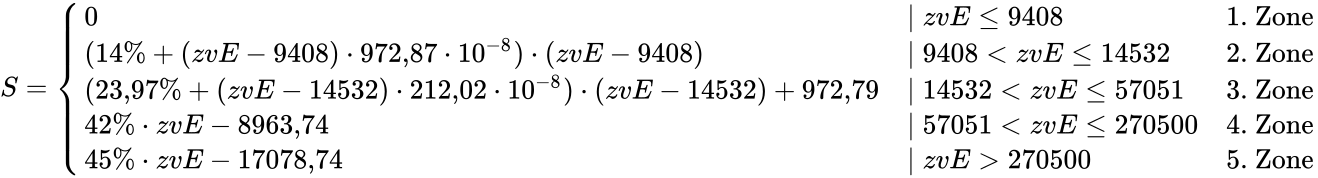
\includegraphics[width=\textwidth]{images/tarifzonen-formel}
						\hfill
					}
					\only<2>{
						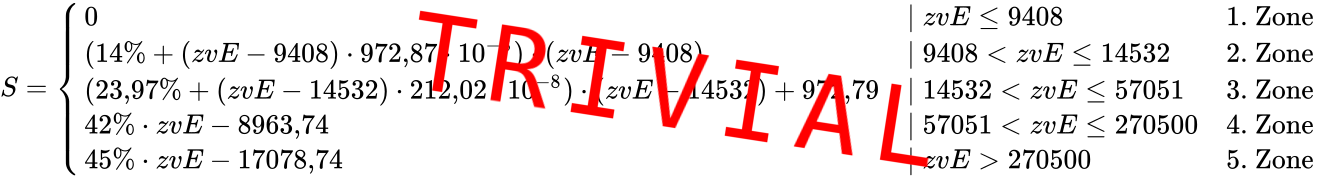
\includegraphics[width=\textwidth]{images/tarifzonen-formel-trivial}
						\hfill
					}
				\end{center}
			\end{frame}
		
			\begin{frame}{Steuersätze}
				\begin{center}
					\vspace{-0.5cm}
					\begin{figure}
						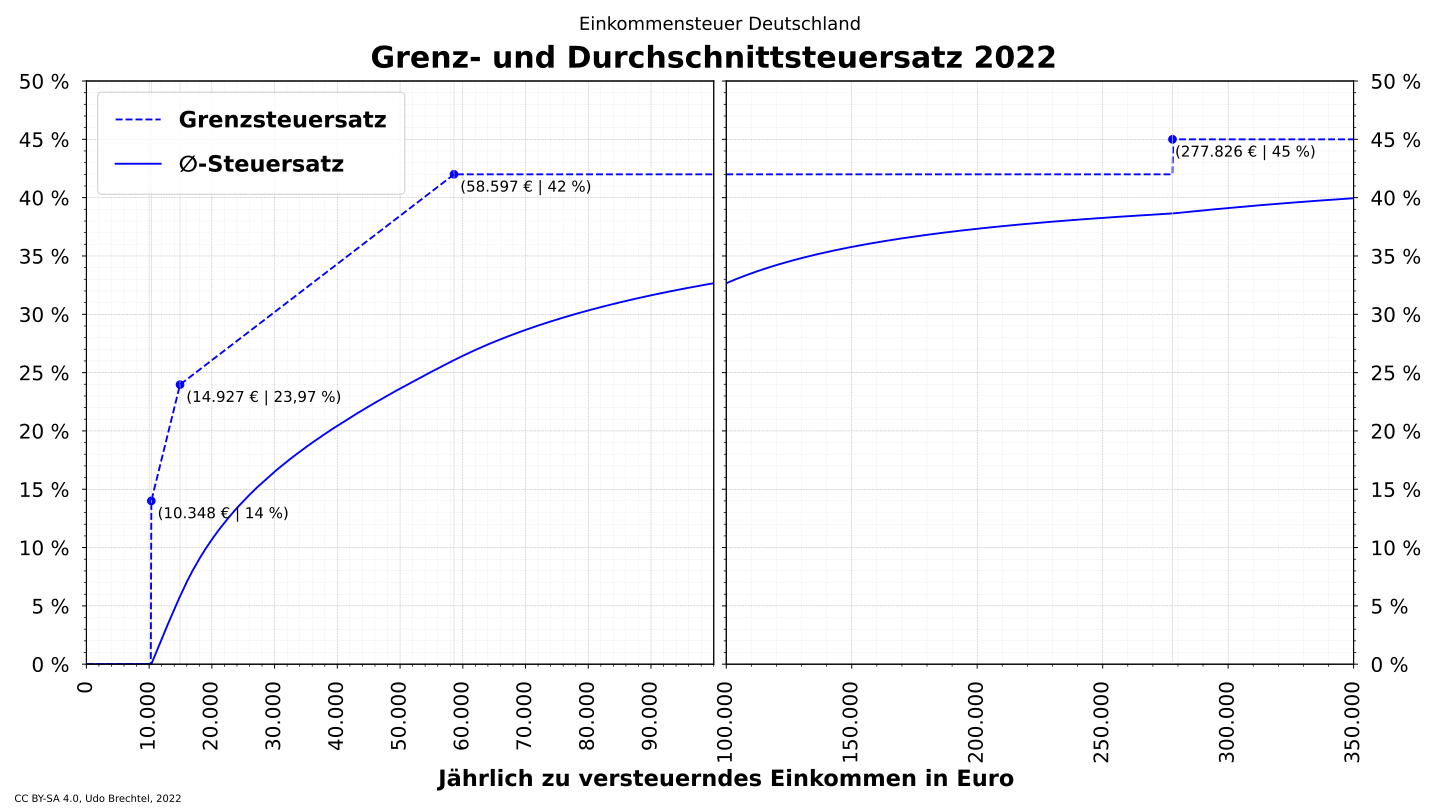
\includegraphics[width=0.9\linewidth]{images/tarifzonen-diagramm}\citeurl{https://commons.wikimedia.org/wiki/File:ESt_D_Tarif_2014_Splitting_120kEUR.svg}{Wikipedia (CC BY-SA 3.0)}
					\end{figure}
				\end{center}
			\end{frame}
			
			\begin{frame}{Arten von\newline Einkommen}
				\begin{center}
					\begin{figure}
						\vspace{-1.5cm}
						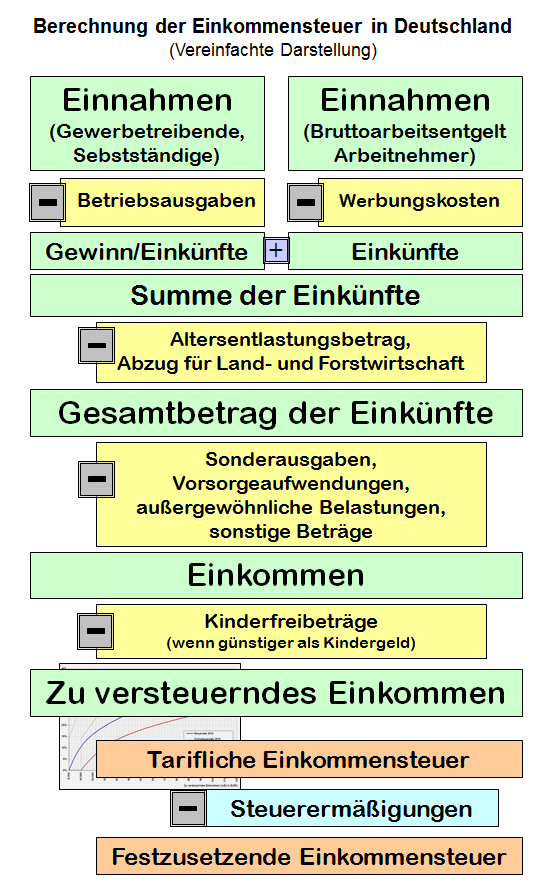
\includegraphics[height=0.9\textheight]{images/zu-versteuerndes-einkommen.png}\citeurl{https://commons.wikimedia.org/wiki/File:Einnahmen_Einkuenfte_Einkommen_zvE.png}{Wikipedia (CC BY-SA 3.0)}
					\end{figure}
				\end{center}
			\end{frame}
			
			\begin{frame}{Einkommen und Steuern}
				\begin{itemize}
					\item Alle Arten von Einnahmen werden besteuert
					\begin{itemize}
						\item Lohn, Verkäufe, Vermietung, ...
					\end{itemize}
					\item \textbf{I.d.R.} überweist Arbeitgeber die Steuer (man selbst braucht nichts tun)
					\item Steuerfreibeträge
					\begin{itemize}
						\item Beispiel Grundfreibetrag: 9984€ in 2022 (832€ / Monat)
					\end{itemize}
					\item Beruflich motivierte Ausgaben \textit{absetzen}
				\end{itemize}
			\end{frame}
		
			\begin{frame}{Von der Steuer absetzen}
				\begin{center}
					
\includegraphics[width=0.75\linewidth]{images/absetzen}
				\end{center}
			\end{frame}
		
			\begin{frame}{Von der Steuer absetzen}
				\begin{itemize}
					\item Finanzamt weiß nur, was du verdienst
					\item Du hast beruflich/steuerlich motivierte Ausgaben?
					\begin{itemize}
						\item Fahrtkosten zum Büro, Monatskarten, ...
						\item Büromaterial, Internet (Home-Office und so), ...
						\item Steuerberater, Lektüre über Steuern, ...
					\end{itemize}
					\item Solche Ausgaben reduzieren das \textit{zu versteuernde Einkommen}
				\end{itemize}\n
				
				\textbf{Fun fact:} Für das Finanzamt sind Ausbildungskosten = beruflich motivierte Kosten.
			\end{frame}
				
			\begin{frame}{Von der Steuer absetzen}
				\textbf{Problem:} Arbeitgeber hat Steuern ja schon gezahlt :(\n
				\textbf{Lösung:} Dem Finanzamt nachträglich über Ausgaben informieren und zu viel gezahlte Steuern zurück bekommen\footnote{PORSCHE CAYMAN S JUNGS! JAWOLL, JAAA! GEIL MAN!}\n
				\textrightarrow\ \textbf{Steuererklärung} :)
			\end{frame}
		
	\section{Studieren und Steuern}
	
		\begin{frame}
			\tableofcontents[currentsection,hideallsubsections]
		\end{frame}
	
		\begin{frame}{Bachelor / Erstausbildung}
			\begin{itemize}
				\item Bachelor = Erstausbildung?
				\begin{itemize}
					\item Meistens ja
					\item Vorher anderes Studium/betriebliche Ausbildung? Dann nein
				\end{itemize}
				\item Absetzen nur als Sonderausgaben (nicht als Werbungskosten)
				\item Max. 6000€ pro Jahr
				\item Verlust/Ausgaben nicht übertragbar auf spätere Jahre
			\end{itemize}
		\end{frame}
	
		\begin{frame}{Master / Zweitausbildung}
			\begin{itemize}
				\item Master = Zweitausbildung!
				\item Absetzen als Werbungskosten
				\item Unbegrenzt viel
				\item Verlust/Ausgaben übertragbar auf spätere Jahre
				\item Mehr Möglichkeiten (z.B. Verpflegungsmehraufwendungen)
			\end{itemize}
		\end{frame}
	
		\begin{frame}{Was kann ich absetzen?}
			Kosten deines Studiums sind (anteilig) absetzbar.\n
			\begin{itemize}
				\item Semestergebühren, Kursgebühren, Exkursionen
				\item Kosten für Bücher, Literatur, Leihgebühren, ...
				\item Fahrtkosten + Unterkunft
				\item Spenden (ggf. Mitgliedsbeiträge bei Vereinen)
				\item Arbeitsmittel, Druck-/Bindekosten
				\item Telefon, Internet
				\item Master only (?\footnote{Soweit ich einen Absatz im ELSTER-FAQ richtig verstehe}): Mehraufwendungen für Verpflegung
			\end{itemize}\n
			Siehe auch \href{https://www.elster.de/eportal/helpGlobal?themaGlobal=help_est_ufa_10_2020}{ELSTER-FAQ}.
		\end{frame}
	
		\begin{frame}{BAföG und Steuern}
			\begin{itemize}
				\item BAföG = Zuschuss + Darlehn
				\item Beides steuerfrei \textrightarrow\ Kein Einfluss auf Steuern
				\item Nichts davon ist absetzbar
			\end{itemize}
		\end{frame}
	
	\section{Steuererklärung}
	
		\begin{frame}
			\tableofcontents[currentsection,hideallsubsections]
		\end{frame}
	
		{
		\setbeamertemplate{background canvas}{}
		\begin{frame}[plain]
			\begin{center}
				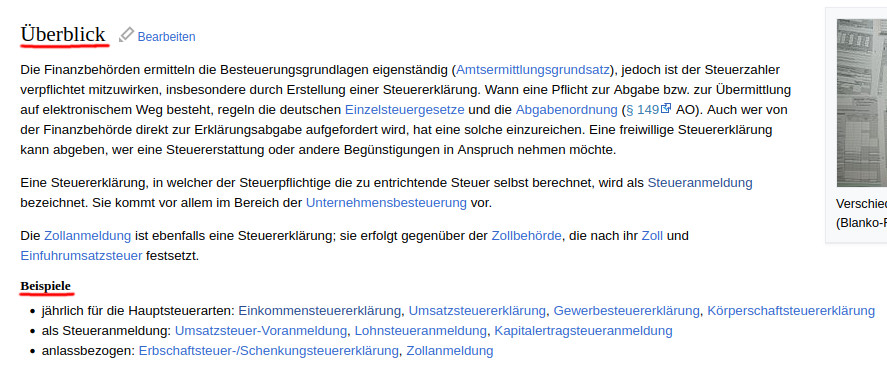
\includegraphics[width=\linewidth]{images/steuererklärung-überblick-1.jpg}
			\end{center}
		\end{frame}
		\begin{frame}[plain]
			\begin{center}
				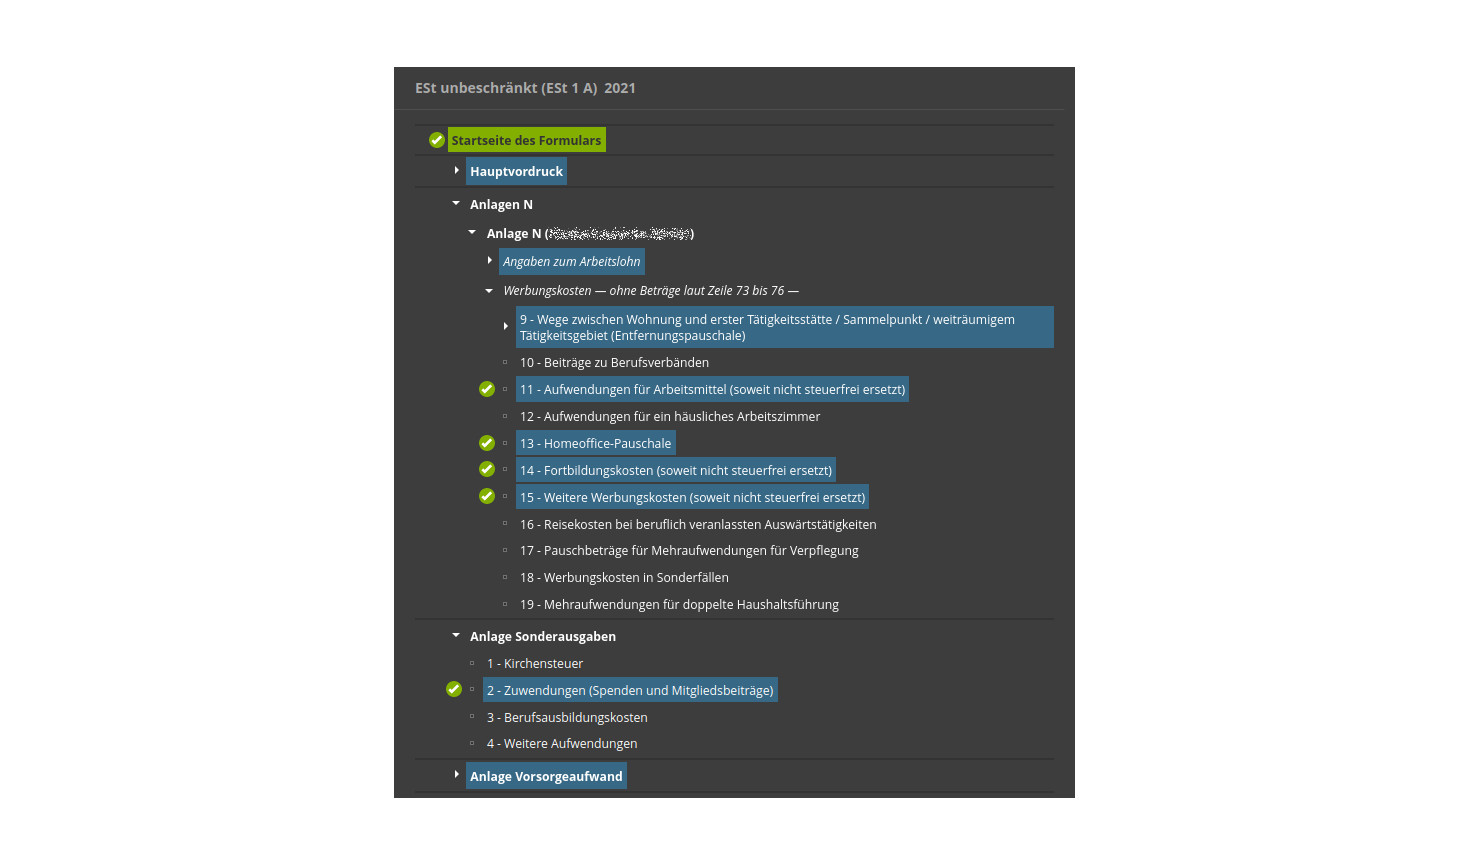
\includegraphics[width=\linewidth]{images/steuererklärung-überblick-2.jpg}
			\end{center}
		\end{frame}
		\begin{frame}[plain]
			\begin{center}
				\includegraphics[height=1.25\textheight]{images/einkommenssteuererklärung-1.jpg}
			\end{center}
		\end{frame}
		\begin{frame}[plain]
			\begin{center}
				\includegraphics[height=1.25\textheight]{images/einkommenssteuererklärung-2.jpg}
			\end{center}
		\end{frame}
		\begin{frame}[plain]
			\begin{center}
				\includegraphics[height=1.25\textheight]{images/einkommenssteuererklärung-3.jpg}
			\end{center}
		\end{frame}
		}

		\subsection{Aller Anfang ist schwer}
		
			\begin{frame}{Wann mache ich meine Steuererklärung?}
				\begin{itemize}
					\item Immer im Folgejahr: Steuererklärung \textbf{für} 2020 macht man also 2021.
				\end{itemize}\n
				\textbf{Fristen:}\\
				\textbf{Angestellt}? \textrightarrow\ freiwillige Abgabe \textrightarrow\ vier Jahre Zeit\\
				\textbf{Selbstständig}/Freiberufler? \textrightarrow\ Pflicht \textrightarrow\ Bis 31. Juli\footnote{Coronabedingt ggf. länger}
			\end{frame}

			\begin{frame}{Wo mache ich meine Steuererklärung?}
				\begin{itemize}
					\item ELSTER\footnote{Elster ... Selbstironie ist der Finanzbehörde nicht fremd.}: Online Dienst der Finanzverwaltung. Hat einen Dark-Mode.
					\item Steuersoftware: Günstig, IMHO selten Mehrwert gegenüber ELSTER
					\item Lohnsteuerhilfeverein: Beratung, mittelmäßig teuer
					\item Steuerberater: Teuer, kann alles für dich machen
				\end{itemize}
			\end{frame}
		
			\begin{frame}{Was brauche ich für meine Steuererklärung?}
				\begin{itemize}
					\item Finanzen, Einnahmen und Ausgaben im Blick haben
					\item Relevante Rechnungen aufheben!
					\item Pauschalen kennen
					\item Fahrten zur Arbeit/Uni notieren
					\item Tage mit mehr als 8h außerhalb merken
				\end{itemize}
			\end{frame}
		
			\begin{frame}{Wie läuft das ab?}
				\begin{itemize}
					\item Jahr endet \& Erhalt Lohnsteuerbescheid
					\item Daten aus Lohnsteuerbescheid in Steuerprogramm eintragen / ggf. automatisch vorausgefüllt
					\item Ausgaben eintragen
					\begin{itemize}
						\item Beruflich/Uni motivierte Kosten
						\item Altersvorsorge, Versicherungen, etc.
						\item Spenden
					\end{itemize}
					\item Abschicken
					\item Ggf. Dokumente (z.B. Rechnungen) nachreichen
					\item Erhalt Steuerbescheid
					\begin{itemize}
						\item Prüfen \& nachvollziehen
						\item Enthält ggf. Erklärungen und Begründungen
					\end{itemize}
				\end{itemize}
			\end{frame}
		
			\begin{frame}{Pauschalen}
				Ohne weitere Nachweise möglich sind:
				\begin{itemize}
					\item Werbungskosten: 1000€
					\item Kontoführung: 16€
					\item Sparerpauschbetrag: max. 801€ auf Kapitalerträge
					\item Home-Office Pauschale: max. 600€
					\item Telefon- \& Internet: max. 20\%\footnote{Mehr ist möglich, dann aber Einzelnachweise nötig} \& max. 20€ pro Monat
					\item Umzug (sofern beruflich motiviert): Uff, also da geht einiges ;)
					\item Entfernungspauschale (s.u.)
					\item Verpflegungspauschale (s.u.)
					\item Arbeitsmittel: 110€\footnote{Mehr ist möglich, dann aber einzeln aufführen} (s.u.)
				\end{itemize}
			\end{frame}
		
		\subsection{Steuererklärung mit ELSTER}
		
			\begin{frame}{Los gehts}
				\begin{enumerate}
					\item Registrierung bei ELSTER
					\item Login
					\item Vorausgefüllte Steuererklärung
				\end{enumerate}
			\end{frame}
		
			\begin{frame}
				\begin{center}
					\vspace{-0.6cm}
					\hspace*{-0.91cm}
					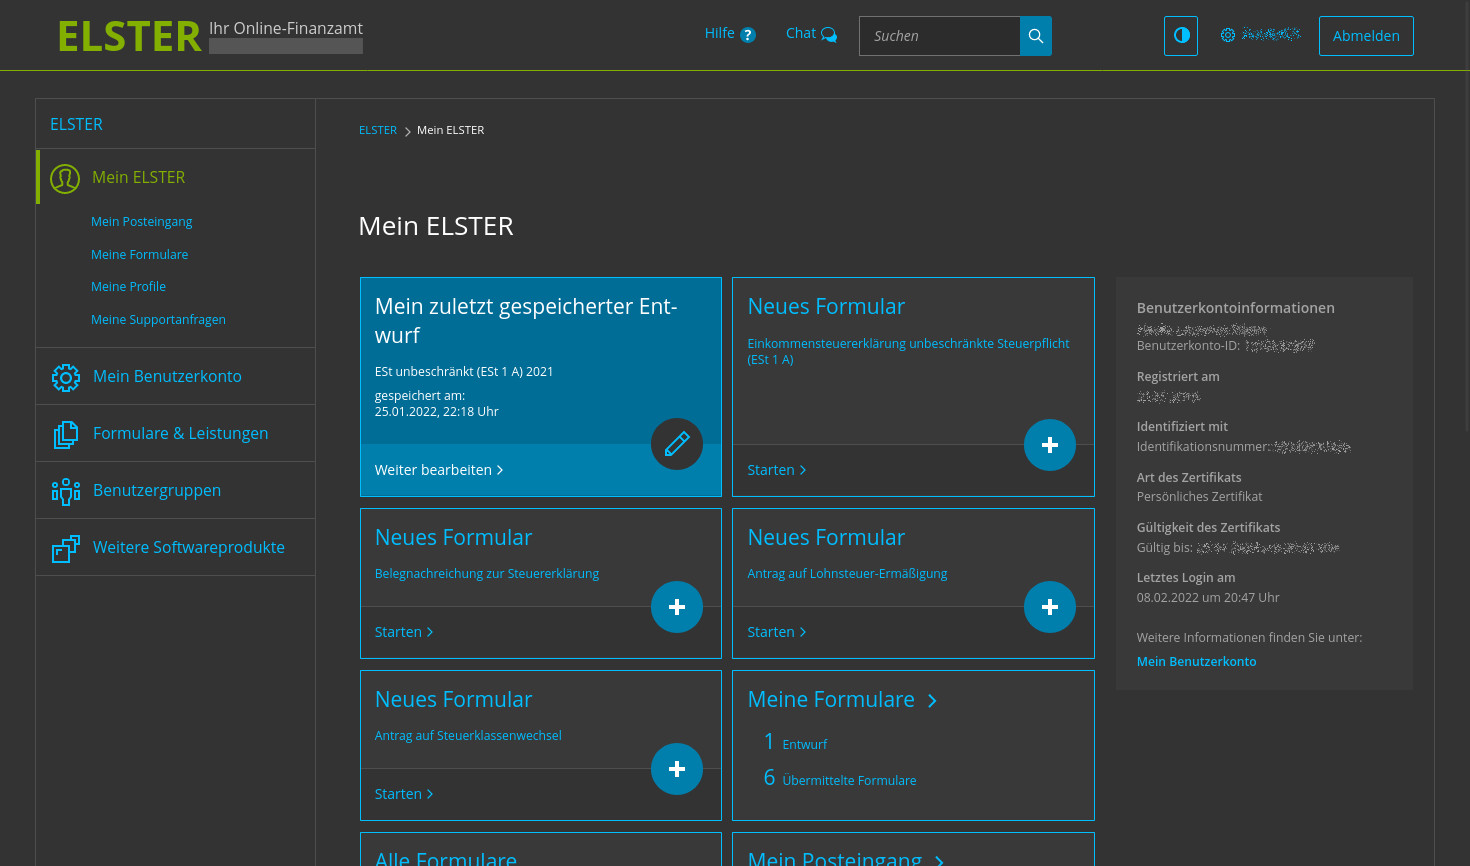
\includegraphics[scale=0.24]{images/elster-1}
				\end{center}
			\end{frame}
		
			\begin{frame}
				\begin{center}
					\vspace{-0.6cm}
					\hspace*{-0.91cm}
					\includegraphics[scale=0.24]{images/elster-übersicht-1}
				\end{center}
			\end{frame}
		
			\begin{frame}
				\begin{center}
					\vspace{-0.6cm}
					\hspace*{-0.91cm}
					\includegraphics[scale=0.24]{images/elster-übersicht-2}
				\end{center}
			\end{frame}
		
		\subsection{Das kannst du absetzen}
		
			\begin{frame}{Home-Office Pauschale}
				\begin{itemize}
					\item 5€ pro Arbeitstag im Home-Office
					\item Max. 600€
					\item In 1000€ Werbungskostenpauschale enthalten
					\begin{itemize}
						\item Beispiel 1: 600€ H.O. Pauschale + 100€ Werbungskosten \textrightarrow\ Werbungskostenpauschale ist größer
						\item Beispiel 2: 600€ H.O. Pauschale + 850€ Werbungskosten = 1450€ \textrightarrow\ 450€ können zusätzlich zur Werbungskostenpauschale abgesetzt werden
					\end{itemize}
				\end{itemize}
			\end{frame}
		
			\begin{frame}{Wege zur Arbeit/Uni}
				Stichwort: Entfernungspauschale / Pendlerpauschale\n
				
				\begin{itemize}
					\item Pro Kilometer 30ct (ab dem 21. Kilometer 35ct bzw. 38ct\footnote{Die 38ct ab dem 21. Kilometer gelten nur für die Jahre 2022 bis 2026})
					\item Einfache Wegstrecke (\textbf{nicht} hin + zurück)
					\item Kilometer werden immer \textbf{ab}gerundet (z.B. 2,9km \textrightarrow\ 2km)
					\item Verkehrsmittel egal: Auto, Fahrrad, Fuß, Fahrgemeinschaft
					\item Zweck muss beruflich sein: Zum Job, zur Uni, zur Lerngruppe (auch bei jemandem Zuhause), zur OE, ...
				\end{itemize}\n
				
				\textbf{Achtung:} Semesterticket wird woanders eingetragen!
			\end{frame}
		
			\begin{frame}{Semesterbeitrag (inkl. Semesterticket)}
				\textbf{Erstausbildung:}\\
				Als Sonderausgaben.\n
				
				\textbf{Zweitausbildung:}\\
				Als Werbungskosten (z.B. unter "`Fortbildungskosten"' oder "`Weitere Werbungskosten"').\n
				\hfill\\
				\textbf{Hinweis:} Entfernungspauschale für Auto, Rad, Fuß geht trotzdem. Steuern sparen durch Rad fahren :D
			\end{frame}
		
			\begin{frame}
				\begin{center}
					\vspace{-0.6cm}
					\hspace*{-0.91cm}
					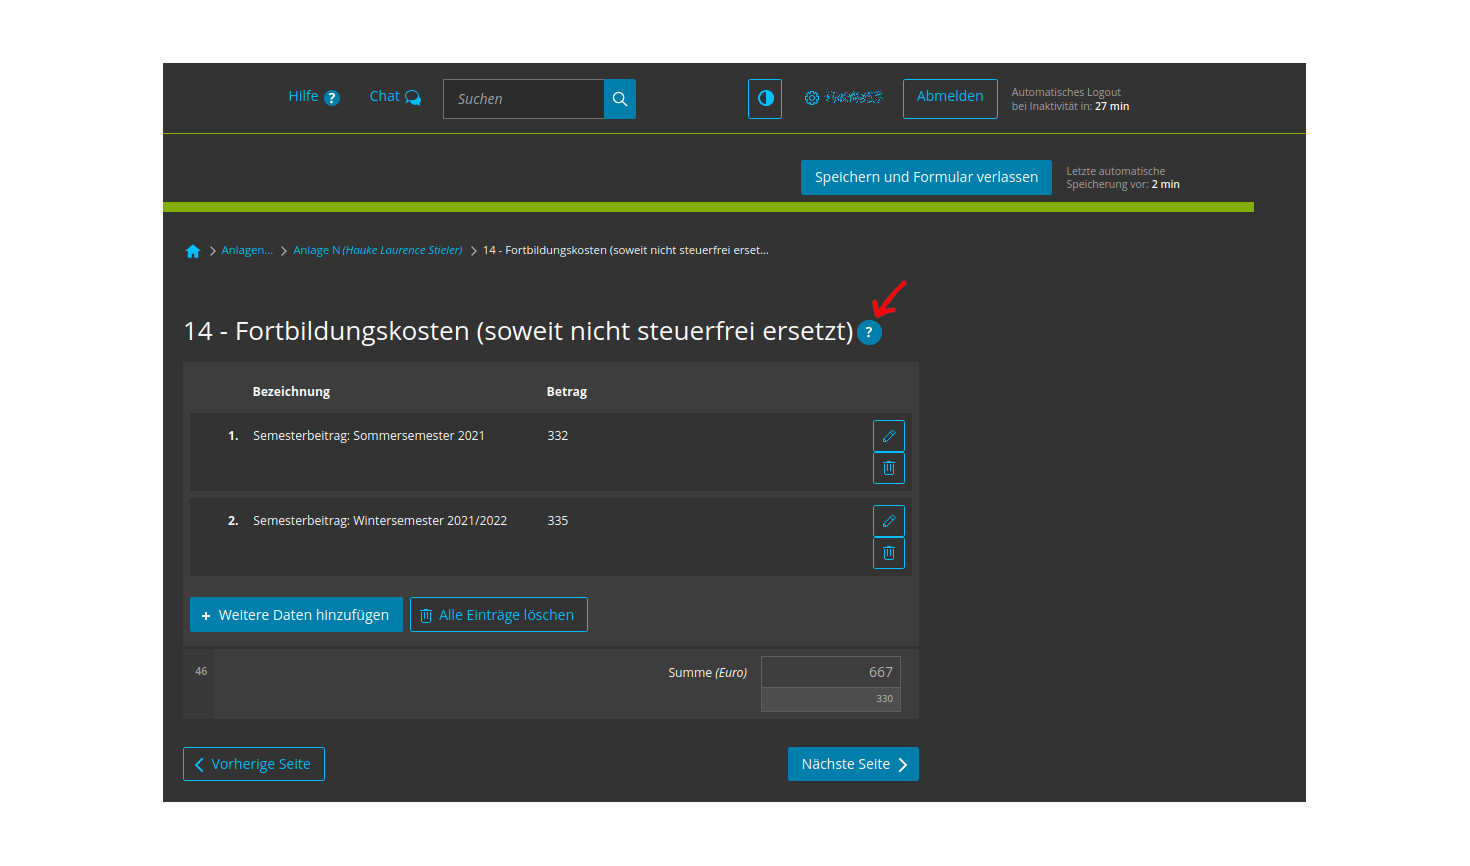
\includegraphics[scale=0.24]{images/elster-fortbildungskosten-1}
				\end{center}
			\end{frame}
			
			\begin{frame}
				\begin{center}
					\vspace{-0.6cm}
					\hspace*{-0.91cm}
					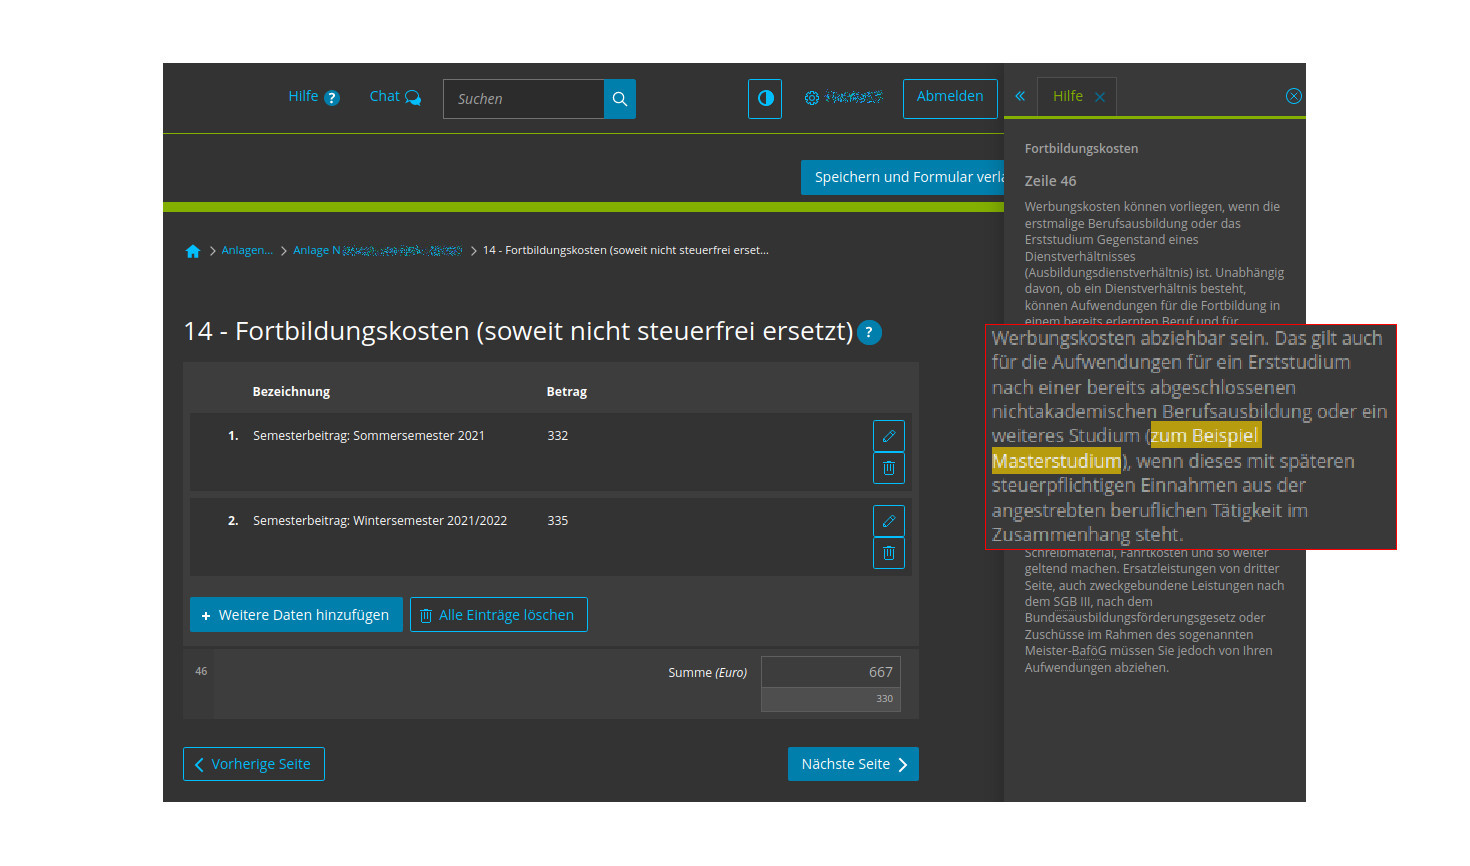
\includegraphics[scale=0.24]{images/elster-fortbildungskosten-2}
				\end{center}
			\end{frame}
			
			\begin{frame}
				\begin{center}
					\vspace{-0.6cm}
					\hspace*{-0.91cm}
					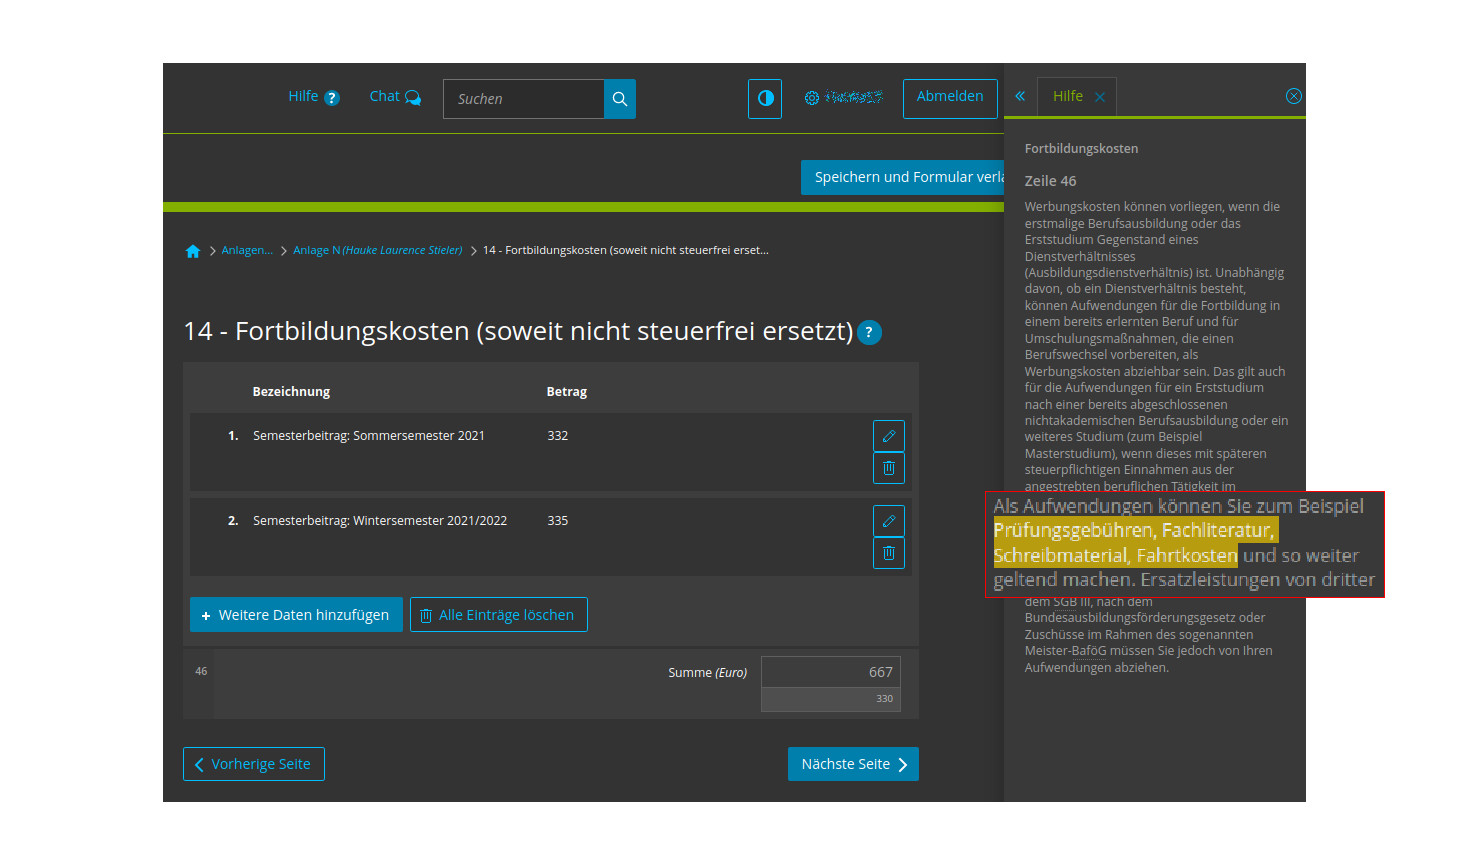
\includegraphics[scale=0.24]{images/elster-fortbildungskosten-3}
				\end{center}
			\end{frame}
		
			\begin{frame}{Verpflegungsmehraufwand}
				Tätigkeit nicht Zuhause \& nicht an erster Tätigkeitsstätte \textrightarrow\ Essen kostet Geld \textrightarrow\ Pauschale für Verpflegung\n
				\textbf{Erste Tätigkeitsstätte:}
				\begin{itemize}
					\item Primärer Ort deiner Tätigkeit (Arbeitnehmer oder Student)
					\item Pro Dienstverhältnis eine erste Tätigkeitsstätte
					\begin{itemize}
						\item Ggf. zwei erste Tätigkeitsstätten (Uni und Arbeitsplatz)
					\end{itemize}
				\end{itemize}\n
				\textbf{Wie absetzen?}
				\begin{itemize}
					\item Tätigkeit außerhalb: Exkursion, Lerngruppe, OE, ...
					\item Mehr als 8h: 12€
					\item Mehr als 24h: 24€ {\tiny \textit{*hust* OEWE / NWE *hust*}}
				\end{itemize}
			\end{frame}
		
			\begin{frame}{Verpflegungsmehraufwand}
				\textbf{Beispiel 1:}\\
				8h in Uni zur Lerngruppe/Vorlesung/... = \textbf{kein} Verpflegungsmehraufwand absetzbar\n
				\textbf{Beispiel 2:}\\
				8h beim Kumpel zum Lernen = Verpflegungsmehraufwand möglich\n
				\textbf{Beispiel 3:}\\
				8h in Bibliothek der UHH die außerhalb des Campus-Teils (z.B. Ikum) ist, in dem man normalerweise studiert und die somit räumlich vom Rest der ersten Tätigkeitsstätte getrennt ist \textrightarrow\ ... keine Ahnung, aber ein Versuch ists wert
			\end{frame}
		
			\begin{frame}{Arbeitsmittel}
				\begin{itemize}
					\item Berufsbekleidung, Equipment, Literatur für den Beruf
					\item Anschaffung, Reparatur, Miete, Reinigung
					\item Mind. 10\% berufliche Nutzung
					\item Kosten anteilig absetzbar
					\item Bis 952€\footnote{800€ Netto + 19\% Mehrwertsteuer}: Im entsprechenden Jahr absetzbar
					\item Über 952€: Verteilung über typische Nutzungsdauer
					\begin{itemize}
						\item Gilt nicht mehr für Computer und Software, die ab 2021 angeschafft wurden!
					\end{itemize}
				\end{itemize}\n
			
				\textbf{Hinweis:} Unbedingt Rechnungen aufheben! Mindestens bis Erhalt des Steuerbescheids, besser ein paar Jahre länger.
			\end{frame}
		
			\begin{frame}{Arbeitsmittel}
				\textbf{Beispiel 1:}\\
				Ich kaufe für 100€ ein Regal und 75\% der Bücher darin sind Fachliteratur \textrightarrow\ 75€ absetzbar.\n
				\textbf{Beispiel 2:}\\
				Ich kaufe eine Tastatur, die ich nur beruflich nutze \textrightarrow\ komplette Kosten kann ich absetzen.\n
				\textbf{Beispiel 3:}\\
				Ich habe nur 90€ für Arbeitsmittel ausgegeben :( \textrightarrow\ Einfach die 110€ Pauschale angeben :)
			\end{frame}
		
			\begin{frame}{Spenden \& Mitgliedsbeiträge}
				Spenden:
				\begin{itemize}
					\item Alles
					\begin{itemize}
						\item Solange Empfänger gemeinnützig, mildtätig oder kirchlich
						\item Empfänger mit Sitz in Deutschland
					\end{itemize}
					\item Bis 300€: Kein Nachweis nötig
					\item Über 300€: Spendenquittung wird ggf. nachgefordert
				\end{itemize}\n
				Mitgliedsbeiträge:
				\begin{itemize}
					\item Ähnliche Regel wie oben
					\item Nicht absetzbar für Sportvereine, Heimatvereine, etc.
				\end{itemize}\n
				\textbf{Wo angeben?} \textrightarrow\ Sonderausgaben
			\end{frame}
		
			\begin{frame}{Aber ich hab gar keinen Job :( \textrightarrow\ Verlustvortrag}
				Du hast Kein Job?\\\pause
				Du machst dein Masterstudium / deine Zweitausbildung?\\\pause
				Trotzdem eine Steuererklärung machen!\n\pause
				\begin{itemize}
					\item Werbungskosten als Verlust ansammeln
					\item Geht nur für Zweitausbildung
					\item In Folgejahren (wenn man Steuern zahlt) anrechnen und dann sparen
				\end{itemize}
			\end{frame}
		
		\subsection{Nochmal in Kürze}
		
			\begin{frame}
				\begin{itemize}
					\item Steruerklärung ohne großen Aufwand online machen
					\item Berufliche/Universitäre Ausgaben können Steuerlast senken
					\item Pauschalen nutzen
					\item Dokumente, Rechnungen, Quittungen, etc. aufheben
				\end{itemize}
			\end{frame}
	
		{
		\setbeamertemplate{background canvas}{}
		\begin{frame}[plain]
			\begin{center}
				
\includegraphics[height=\textheight]{images/too-afraid-to-ask.jpg}
			\end{center}
		\end{frame}
		}
\end{document}













